%%%%%%%%%%%%%%%%%%%%%%%%%%%%%%% TO DOS %%%%%%%%%%%%%%%%%%%%%%%%%%%%%%%
% 1. 
%%%%%%%%%%%%%%%%%%%%%%%%%%%%%%%%%%%%%%%%%%%%%%%%%%%%%%%%%%%%%%%%%%%%%%

\section{Introduction} 
\label{sec:intro}
%%%%%%%%%%%%%%%%%%%%%%%%%%%%%%%%% DCC is here %%%%%%%%%%%%%%%%%%%%%%%%%%%%%%%%%%
Today's datacenters (DCs) are server-centric: users rent servers with
specific hardware capabilities tailored to their needs (e.g.,
compute-intensive EC2 instances from Amazon). 
A \emph{disaggregated} datacenter (DDC) disaggregates, or separates,
the resources in a traditional DC into resource \emph{blades},
with each resource connected directly to an interconnect (Figure~\ref{fig:DDC}). 
We use the term \emph{blade} to describe a 1U server containing one resource
type, and \emph{resource} for an individual CPU, DIMM, SSD, etc. in a blade. 

%%%%%%%%%%%%%%%%%%%%%%%%%%%%%%%%% DDC benefits %%%%%%%%%%%%%%%%%%%%%%%%%%%%%%%%%

% The modularity of DDCs benefits both operators and
% users~\cite{Han2013}. By separating resources into blades, a
% DDC provides efficiency: the operator can upgrade specific hardware
% blades without impacting other resources types. Users also experience
% an efficiency win: in a DDC a user can provision the exact amount of
% resources they require and dynamically expand/shrink this set. This flexibility
% also increases the DC resource utilization.

%%%%%%%%%%%%%%%%%%%%%%%%%%%%% Research challenges %%%%%%%%%%%%%%%%%%%%%%%%%%%%%%

% There are two broad types of disaggregation: partial and full.
% In partial disaggregation compute resources have a small amount of local memory,
% memory and storage resources have CPUs, and a NIC is attached to each resource. 
% In full disaggregation each resource is independent and is directly
% connected to the rack interconnect. Current research focuses on the practicality
% of partial disaggregation~\cite{IntelRSA,Gao2016,Lim2009,Lim2012}.

% In this paper, we discuss partial disaggregation at rack-scale:
% resources can only connect to other resources in the same rack (e.g., a CPU in
% rack1 cannot connect to a DIMM in rack2). The disaggregated rack is presented to
% the client as a single machine through a virtualization layer. Applications can
% request a number of VMs to allocate among the racks. Distributed applications
% might then run among several disaggregated racks, while a single-machine
% application will reside in one rack.

Disaggregation challenges several assumptions behind datacenter software
design: as memory becomes rack-wide and shared between disaggregated CPUs, the
entire rack resembles a ccNUMA system rather than a set of traditional
distinct servers. 
% This resemblance now allows applications to have access to a
% globally shared address space, potentially providing performance wins for data
% intensive applications.
The idea of a globally shared address space is not new~\cite{Nelson2015,Keleher1994}.
Although distributed global address spaces have advantages (single-host
applications can scale to clusters and operate on data with a global view),
they historically do not gain traction due to the implications of transparent
distribution: poor performance and difficult to understand failure models. 

% ccNUMA machines also encounter these same issues unless applications are
% written explicitly for non-uniform access of memory. Scalable
% single-host systems are often designed with each core acting as a
% ``shared-nothing'' instance. Essentially, each core operates independently on
% partitioned data and local structures. 

Yet, with the emergence of disaggregation, the implementation of global shared
memory systems should be revisited in this new context. More specifically, we
plan to address the question: \emph{How can we design a system that will
present a rack of disaggregated resources like a supercomputer?} To do so, we
plan on extending the \texttt{BlueBridge} distributed memory system in four
ways. We will add support for remote memory sharing and memory RAIDing to
provide a resilient globally shared address space. We will also optimize the
user space paging and implement different cache eviction policies to reduce
latency on the end hosts. Finally, we will add a programmable switch which acts
as the memory controller for the address space. We believe by moving the memory
controller from the end-host to the network switch, we will reduce the overhead
of memory RAIDing, allocation, and paging.


%%%%%%%%%%%%%%%%%%%%%%%%%%%%%%%%%%%%%%%%%%%%%%%%%%%%%%%%%%%%%%%%%%%%%%%%%%%%%%%%
\begin{figure}
    \centering
    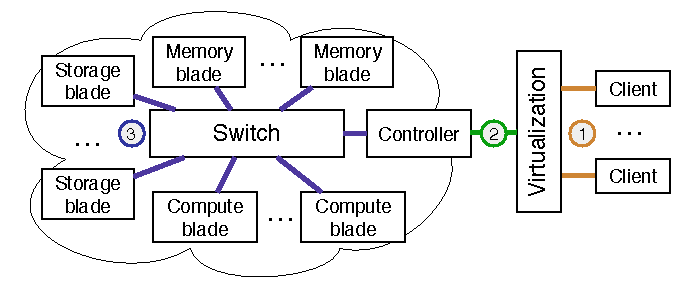
\includegraphics[width=\columnwidth]{fig/ddc-overview}
    \caption{Simplified representation of a disaggregated datacenter with
    three communication points: (1) between the application and the
    virtualization layer,
    (2) between the virtualization layer and the physical resources, and (3)
    between the physical resources bundled as blades.}
    \label{fig:DDC}
\end{figure}
%%%%%%%%%%%%%%%%%%%%%%%%%%%%%%%%%%%%%%%%%%%%%%%%%%%%%%%%%%%%%%%%%%%%%%%%%%%%%%%%
